\chapter{Marco teórico}

En este capítulo se presentan, de forma teórica, los conceptos y técnicas
necesarias para el desarrollo de este proyecto. Se comienza por delimitar
la problemática en el marco del NLP, posteriormente se presentan los
modelos de lenguaje y su aplicación a la problemática, así como la
descripción de la técnica de recuperación-generación aumentada que se empleará,
además de conceptos adicionales necesarios para el desarrollo del proyecto,
por último se presentan trabajos relacionados en el área.

\section{Delimitación de la problemática}

El objetivo de este proyecto es desarrollar un asistente virtual tipo chatbot
que responda preguntas de documentos específicos. Si bien, un asistente
virtual inteligente se desempeña en diferentes áreas del NLP, este proyecto
se centra específicamente en el que se conoce como dar respuesta a preguntas
(QA, Question Answering).

En el contexto del NLP, se entiende como QA al desarrollo de sistemas que
permiten a usuarios emplear interfaces de lenguaje natural para realizar
preguntas y recibir respuestas concisas \cite{pereira_systematic_2022}.
Estos sistemas pueden presentarse de diferentes formas, sin embargo,
actualmente son los modelos de lenguaje de gran tamaño (LLMs) los que
predominan en el área y hacen posible la creación de sistemas que responden
a preguntas de forma interactiva (IQA, Interactive Question Answering),
donde el sistema puede entablar conversaciones con el usuario y responder
las preguntas de forma dinámica \cite{biancofiore_interactive_2024}.

Una parte importante del QA es que, generalmente, funciona con ternas de
información: pregunta, contexto, respuesta. La pregunta y la respuesta
son secuencias de texto en lenguaje natural, y el contexto se refiere a
la información que empleará el modelo para contestar la pregunta, usualmente
el contexto también se encuentra en forma de texto, aunque puede tener
otras formas.

Dentro de los sistemas IQA y QA, existen diferentes elementos a evaluar,
sin embargo la evaluación de la respuesta es el parámetro fundamental en la
mayoría de ellos, para ello se emplean datasets especializados que contienen
preguntas, su contexto y las respectivas respuestas, por ejemplo:
TREC (\textbf{T}ext \textbf{RE}trieval \textbf{C}onference)
\cite{noauthor_proceedings_2001}, Yahoo! (YH) \cite{zhou_learning_2016},
WikiQA \cite{yang_wikiqa_2015}, Standford Question Answering Dataset (SQuAD)
\cite{rajpurkar_squad_2016}, entre otras.


\section{Modelos de lenguaje de gran tamaño (LLMs)}

Para entender lo que es un LLM, primero es necesario presentar el concepto
de red neuronal artificial (ANN, Artificial Neural Network).
Una red neuronal artificial es un modelo dividido en capas de
procesamiento, donde cada capa se compone de nodos o neuronas. Cada neurona
recibe entradas ponderadas, les aplica una transformación y devuelve una
salida. En el modelo tradicional de red neuronal, conocido como
\textit{feedforward}, las salidas de cada capa sirven como entrada de la
siguiente, de esta forma la información se propaga
desde la capa de entrada, pasando por una o más capas ocultas hasta llegar
a la capa de salida, donde se obtiene el resultado final de la red.

Múltiples arquitecturas de ANNs han sido creadas con diferentes propósitos,
y a su vez, se han creado mecanismos que funcionan en conjunto con estas
redes para mejorar su desempeño en tareas específicas. En el contexto del
NLP uno de estos mecanismos es la \textit{atención}. Este mecanismo
fue introducido por Bahdanau et al. \cite{bahdanau_neural_2016} en el contexto
de la traducción de textos automática con el propósito de que una red neuronal
pudiera decidir a qué partes de las oraciones prestar atención.
Si bien Bahdanau no empleaba el término \textit{atención}, su propuesta fue
tomada por Vashwani et al. \cite{vaswani_attention_2017} para crear la
arquitectura del \textit{transformer} para crear una arquitectura basada
únicamente en mecanismos de atención la cual se muestra en la figura
\ref{fig:transformer}.

\begin{figure}[]
    \centering
    \includegraphics[width = 0.5\textwidth]{\DirFigCdos/transformer}
    \caption{Arquitectura \textit{transformer}. **Cambiar por diagrama en español**}
    \label{fig:transformer}
\end{figure}

El \textit{transformer} esta basado en una arquitectura del tipo
codificador-decodificador, es decir, una red neuronal divida en dos partes
cuyo objetivo es convertir una secuencia de texto a otra.

En su artículo, Vashwani define una función de atención como un mapeo de una
\textit{query} y un conjunto de pares \textit{key}-\textit{value} a una salida,
donde la \textit{query}, las \textit{keys} y los \textit{values} son vectores.
Esta salida es una suma ponderada de los \textit{values}, donde el peso
asignado a cada \textit{value} es calculado por una función de compatibilidad de la
\textit{query} con la \textit{key} correspondiente. Para realizar este
cálculo de forma eficiente se emplea el \textit{Scaled Dot-Product Attention}
definido en la ecuación \ref{eq:attention}.

\begin{equation}\label{eq:attention}
    Attention(Q,K,V) = softmax(\frac{QK^T}{\sqrt{d_k}})V
\end{equation}

Esta operación puede replicarse de forma paralela, con el objetivo de que el
modelo preste atención a información de diferentes representaciones de
subespacios en diferentes posiciones, conformando lo que se denomina
\textit{Multi-Head Attention}, definido por la ecuación \ref{eq:multi_attention}.

\begin{equation}\label{eq:multi_attention}
    \begin{split}
        MultiHead(Q,K,V) = Concat(head_i, ..., head_h)W^O \\
        \text{where } head_i = Attention(QW_i^Q, KW_i^K, VW_i^V)
    \end{split}
\end{equation}

Estos bloques de atención son replicados y combinados en la estructura de
codificador-decodificador, dando como resultado la arquitectura del transformer.
Es de esta arquitectura, que derivan múltiples modelos
con arquitecturas profundas cuyo propósito es realizar tareas relacionadas
con el NLP, a estos modelos se les conoce como LLMs.

\section{\textit{Transformers} pre-entrenados}

Los modelos actuales basados en \textit{transformers} son entrenados de forma
general en dos etapas: Un pre-entrenamiento no supervidado en un corpus
muy grande de texto para hacer modelado de lenguaje estándar, seguido de
un ajuste fino supervisado en tareas específicas empleando datasets
especializados y modificando solamente la salida del modelo. Esta forma de
entrenamiento fue propuesta por Radford et al. \cite{radford_improving_2018},
la cual combinada con el uso de una arquitectura de transformer decodificador
\cite{liu_generating_2018} es la base de los LLM actuales y los empleados en
este proyecto.

\section{Modelos multidominio}

En la actualidad existen LLMs que, además de ser \textit{transformers}
pre-entrenados, pasan por diferentes etapas de ajuste fino, reentrenamiento
en múltiples tareas de diferentes dominios, moderación de respuestas, entre
otras, y además de poseen capacidades conversacionales, como es el caso de
ChatGPT (OpenAI), Gemini (Google), Llama (Meta), entre otros.
Estos modelos, al combinarse con interfaces de usuario amigables y
elementos de aplicaciones comerciales permiten realizar una multitud de
tareas directa o indirectamente relacionadas con NLP, siendo una de ellas
la respuesta a preguntas desde documentos.

Los modelos multidominio, al ser arquitecturas profundas, usualmente se
relacionan con su número de parámetros como métrica de su tamaño, estando
por lo general en el orden de billones. Esta medida es importante pues
sirve para determinar la cantidad aproximada de memoria de video que requieren
para funcionar en su modo de inferencia de acuerdo a la ecuación
\ref{eq:params_to_vram}.

\begin{equation}\label{eq:params_to_vram}
    VRAM(bytes) \approx N_{params} \times \text{bytes-per-param} \times (1 + \alpha)
\end{equation}

\section{Modelos de representaciones vectoriales \textit{embeddings}}

Se llama \textit{embedding} a una representación numérica de una secuencia de
caracteres, que puede ser una palabra o una oración completa. La característica
principal de un \textit{embedding} es que las palabras similares tienen
\textit{embeddings} similares, mientras que palabras u oraciones diferentes u
opuestas tienen \textit{embeddings} muy distintos.

Los modelos con la capacidad de generar representaciones con estas
características se conocen como modelos de \textit{embeddings}. Particularmente,
el modelo SBERT fue creado con este propósito y tiene la característica de
que funciona para oraciones completas de texto, y no solo con palabras.
Otro ejemplo es el modelo Qwen3-Embedding.

\section{Modelos comerciales}

Se entiende por modelos comerciales a aquellos que pertenecen a una entidad
privada y su uso está restringido por el pago de una subscripción.
Además, la arquitectura del modelo, métodos de entrenamiento, así como sus
parámetros de funcionamiento no son públicos. Algunos ejemplos son ChatGPT
(OpenAI), Gemini (Google), Claude (Anthropic), entre otros. Usualmente los
proveedores de estos modelos lo hacen a través de aplicaciones web o APIs,
y en ocasiones, cuentan con versiones gratuitas con capacidades limitadas.

\section{Modelos de código abierto}

Los modelos de código abierto son aquellos que se encuentran disponibles
en sitios especializados, tanto su arquitectura como parámetros de
funcionamiento son accesibles, usualmente a través de una licencia de uso
que usualmente no es restrictiva. Algunos ejemplos son DeepSeek (DeepSeek),
Llama (Meta), Qwen (Qwen), entre otros. Los creadores de estos modelos
generalmente no proveen aplicaciones web o APIs, sino que permiten que los
usuarios o desarrolladores los utilicen en sus propias infraestructuras,
sin depender del creador.

\section{QA con modelos multidominio}

Un modelo multidominio tiene la capacidad de responder preguntas que se
le hagan en lenguaje natural. Para emitir una respuesta lo puede hacer de
diferentes formas.

\subsection{Respuestas desde conocimiento previo}

Durante el entrenamiento del modelo, éste se entrena con corpus de información
muy grande y de diversas fuentes, además de que se le hace un ajuste fino
para esta tarea, de tal forma que el modelo es capaz de responder una pregunta
utilizando la información que se le proporcionó durante su entrenamiento.

Este tipo de respuestas es buena cuando se trata de preguntas de dominio abierto
donde la información es pública y no cambia con el tiempo, como es el caso
de conocimientos generales o eventos históricos.

Sin embargo, las respuestas suelen ser deficientes
cuando se trata de eventos recientes, situaciones personales o conocimiento
restringido, en estos casos se pueden presentar alucinaciones, que son
respuestas cuya estructura es correcta, pero su información es errónea.

Otra limitante es que aunque la respuesta sea correcta, generalmente los
modelos no cuentan con la capacidad de indicar la fuente de la información.

\subsection{Respuestas desde un contexto}

En situaciones donde el modelo no tiene forma de conocer la respuesta porque
no fue entrenado con esa información, es posible proporcionarle un contexto
desde el cual el modelo pueda buscar o inferir la respuesta. Este contexto
usualmente es en forma de texto aunque puede tener otras formas y debe contener
la respuesta. Un ejemplo es proporcionar la información bibliográfica de una
persona como contexto y hacer preguntas sobre la persona o relatar una
situación para hacer una pregunta específica.

Generalmente, estas respuestas son más acertadas, pues los modelos son entrenados
en este tipo de tareas, siempre y cuando el contexto sea adecuado. Una
desventaja de este método es que los modelos operan con ventanas de contexto
limitadas, las cuales pueden ser de algunos miles de tokens hasta unos pocos
millones y es posible que el contexto que se deba proporcionar sea mayor.

\section{Recuperación-Generación Aumentada}

Para superar las limitantes que presentan los LLMs, el uso de técnias de
de Recuperación-Generación Aumentada (RAG, Retrieval-Augmente Generation) ha
sido incorporado con frecuencia. Estas técnicas consisten en incorporar
información o conocimiento desde fuentes de datos externas, que sirven como
complemento a las preguntas \cite{fan_survey_2024}.

Un esquema de RAG simple, como el quese presenta en la figura \ref{fig:rag}
contempla tres etapas principales: Indexado, Recuperación y Generación

\begin{figure}[]
    \centering
    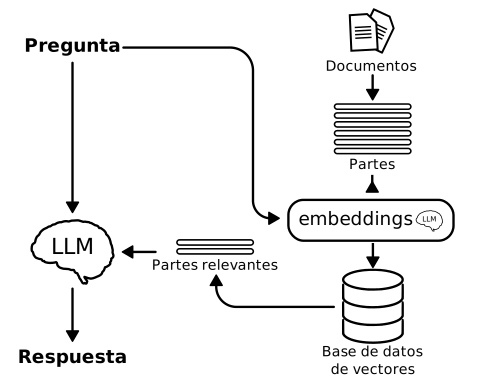
\includegraphics[width = 0.5\textwidth]{\DirFigCdos/simple_rag}
    \caption{Diagrama de funcionamiento de un esquema de RAG simple.}
    \label{fig:rag}
\end{figure}

\subsection{Indexado}

En su forma más simple, una base de conocimiento para RAG parte de la recolección
de documentos relacionados con las preguntas posteriores. Una de las ventajas
es que no hay limitante en la cantidad o tamaño, aunque si deben estar en
formato de texto. Estos documentos se separan en framentos, comunmente
llamados \textit{chunks}, el objetivo es obtener fragmentos pequeños pero
que contengan suficiente información. Posteriormente se calcula la
representación vectoriale (\textit{embedding}) de cada framento, para finalmente
almacenar cada fragmento con su respectivo \textit{embedding} en una base
de datos.

\subsection{Recuperación}

Dada una solicitud hecha al LLM, la recuperación consiste
en buscar información relevante, usualmente en forma de fragmentos de
documentos, en una base de datos previamente construida. La forma de
determinar si un fragmento es relevante o no para la pregunta se mide la
distancia entre la solicitud y el fragmento.

Una de las formas más comunes de medir esta distancia es empleando la
distancia coseno, en su forma de similitud coseno, como se muestra en la
ecuación \ref{eq:cos_similarity}

\begin{equation}\label{eq:cos_similarity}
    d = 1.0 - \frac{\sum{(A_i \times B_i)}}{\sqrt{\sum{(A_i^2)}}\sqrt{\sum{(B_i^2)}}}
\end{equation}

Otra de las métricas comunes es la distancia empleando el producto interno,
como se muestra en la ecuación \ref{eq:inner_product}.

\begin{equation}\label{eq:inner_product}
    d = 1.0 - \sum{(A_i \times B_i)}
\end{equation}

\subsection{Generación}

En esta etapa, tanto la solicitud como los documentos seleccionados son
sintetizados en una instrucción coherente que se le proporciona al modelo.
Usualmente esta instrucción incluye: Indicación de responder la pregunta
solamente con los fragmentos proporcionados, los fragmentos de texto y la
pregunta.

\section{Reentrenamiento de los modelos}

Tanto los LLMs comerciales como los de código abierto pasan por una serie de
pasos de entrenamiento y ajuste para funcionar adecuadamente en los
diferentes dominios para los que son preparados, de esta forma pueden ser
utilizados directamente sin modificaciones, sin embargo, en ocasiones es
posible mejorar su rendimiento en tareas específicas aplicando diferentes
técnicas de ajuste.

\subsection{Ingeniería de instrucciones (\textit{prompts})}

Cuando un modelo está entrenado para seguir instrucciones, es posible modificar
su comportamiento dando instrucciones adicionales que le sirvan como guía
al momento de dar la respuesta, a esto se le conoce como ingeniería de prompts.

Con esta técnica se puede instruir al modelo a realizar una serie de pasos
antes de dar la respuesta, modificar el tono, longitud o intención de la
respuesta, además de proporcionar información sobre la situación en que
se debe desempeñar.

\subsection{Ajuste fino supervisado}

Consiste en tomar un dataset que contenga ejemplos del comportamiento que
se desea que aprenda el modelo, en este proceso suelen usarse
ejemplos con pares intrucción-respuesta, donde la respuesta tiene
las características que se desea que el modelo aprenda. En este proceso
solo la salida del modelo es modificada, mientras todo lo demás permanece
igual, lo cual permite reducir la cantidad de recursos necesarios.

\subsection{Aprendizaje por refuerzo}

El aprendizaje profundo consiste en entrenar al modelo para tomar decisiones
que maximicen una recompenza. En el caso de los modelos de lenguaje, uno
de los enfoques más utilizados es el aprendizaje por refuerzo con
retroalimentación humana (RLHF, Reinforcement Learning from Human Feedback),
el cual utiliza retroalimentación humana para optimizar modelos.

Esta técnica de ajuste es particularmente útil porque es posible hacer que
el modelo adquiera comportamientos que no son fáciles de modelar matemáticamente,
sin embargo, tiene la desventaja de que requiere intervención humana y es por
ello más lento.

\section{Documentos normativos}

Se entiende como documentos normativos a aquellos que contienen reglas o
normas que rigen la operación de una organización o un organismo dentro de la
misma, también pueden ser reglamentos de eventos o actividades específicas.

En la actualidad, la mayoría de los documentos normativos de cualquier
organización se encuentran digitalizados en formato PDF y, en ocasiones, disponibles
en servidores web para que los miembros de las organizaciones puedan consultarlos
en cualquier momento.

En el caso de la normativa de la Universidad de Guanajuato, y de muchas otras
normativas, la estructura de los documentos se divide principalmente en:
Título, Sección, Capítulo y Artículos. Este trabajo pretende aprovechar esta
estructura predefinida para referenciar las repuestas del sistema.

\subsection{Formato PDF}

El formato PDF (Portable Document Format) es un formato cuyo objetvio es
ofrecer una forma sencilla y segura de presentar e intercambiar documentos con
independencia del software, el hardware o el sistema operativo que utilice quien
los consulte, con este fin, se encuentra estandarizado por la
ISO (Organización Internacional de Normalización) bajo la ISO 32000-1:2008
(PDF 1.7) y más recientemente la ISO 32000-2:2020 (PDF 2.0) [cita ISO].

Sin embargo, el formato PDF fue pensado como una herramienta para presentar
documentos en una forma entendible por humanos, es decir, no está
diseñado para que una máquina interprete su contenido de forma fácil, sino
para que un humano lo haga.

\subsection{Herramientas de extracción de texto}

Los LLMs operan con entradas de texto, si los documentos a ser empleados
se encuentran en formato PDF es necesario extraer la información textual que
contienen, para ello existen diferentes herramientas, sin embargo, el
resultado suele presentar errores errores o limitaciones propias del formato
PDF, como son la presencia de encabezados y pies de página entre el contenido
del documento, la falta de información sobre títulos, subtítulos o divisiones
de secciones, la dificultad para leer tablas, entre otras.

En el Apéndice A se encuentra una lista de las herramientas más comunes y
sus limitantes, la cual se emplea para seleccionar la herramienta más apta.

Dependiendo de la herramienta a emplear se debe hacer un procesamiento del
archivo PDF para eliminar los defectos e información que no sea relevante,
este proceso se presenta como parte de la metodología del proyecto.

\section{Trabajos relacionados}

En un esfuerzo por implementar una arquitectura robusta para hacer QA
desde diferentes fuentes de inforamción, Christmann \& Weikum
\cite{christmann_rag-based_2024} presentaron el sistema QUASAR, el cual emplea una
arquitectura basada en RAG para responder preguntas desde texto sin estructura,
tablas y grafos de conocimiento. Este sistema procesa las preguntas en
diferentes etapas, que denomina: Entendimiento de la pregunta, recuperación
de evidencia y reclasificación y filtrado. Con esta metología alcanzó
resultados superiores a modelos grandes como GPT-4 y Llama 3 en los benchmarks
CompMix \cite{christmann_compmix_2024} y TimeQuestions \cite{jia_complex_2021}
con un modelo Llama 3.1-8B-instruct
\footnote{https://huggingface.co/meta-llama/Llama-3.1-8B-Instruct}.

Al ser sistemas basados en RAG, nuestro sistema comparte elementos comunes
con el sistema QUASAR, sin embargo, nuestro trabajo pretende aprovechar
la estructura semi-estandarizada de los documentos normativos para realizar
una separación más eficiente de los documentos, además, la restricción
del dominio de las preguntas a documentos específicos, permite construir
una base de datos de conocimiento más sencilla, tanto en tamaño como en
pasos de procesamiento, lo que generaría un sistema más rápido y compacto.

Uno de los problemas principales del RAG es la recuperación de fragmentos
relevantes de los documentos, trabajos como el de Shao et al. \cite{shao_enhancing_2023}
se centran en proponer mejores técnias en la identificación de
documentos relevantes en cuerpos muy grandes de datos aplicando una
sinergia entre el recuperador y el generador para mejorar la respuesta
de forma iterativa. Otra forma de atender este problema lo presenta
Shi et al. con su framework RePlug \cite{shi_replug_2024}
el cual consiste en tratar al modelo de lenguaje que responde la pregunta
como un modelo de caja negra, mientras que el recuperador de información
es el que se entrena y ajusta, de esta forma mejora la capacidad de
QA del modelo sin tener que reentrenarlo. Es por esas consideraciones
que el sistema que se propone en este proyecto considera una etapa de ajuste
fino para el modelo que obtiene los \textit{embeddings} de los documentos,
el cual funciona como recuperador.

Por último, existen herramientas comerciales y de código abierto con la
capacidad de ejecutar metodologías RAG para responder a preguntas de documentos,
siendo el más usado ChatGPT
\footnote{https://help.openai.com/en/articles/8868588-retrieval-augmented-generation-rag-and-semantic-search-for-gpts},
el cual permite generar chats personalizados
y proporcionar una serie de documentos como contexto, al habilitar la opción
de "Recuperación de conocimiento", la herramienta aplica RAG y responde
las preguntas correspondientes. Otra heramienta con características
similares es LMStudio
\footnote{https://lmstudio.ai/docs/app/basics/rag},
la cual es de código abierto y permite el uso de
diferentes modelos, así como su ejecución en entornos locales.

A pesar de las bondades de las herramientas existentes, éstas
ponen sobre el usuario la responsabilidad de encontrar los documentos
requeridos y proporcionarlos a la herramienta, además tienen un límite de
documentos a subir y cuando el chat crece mucho, se debe reiniciar y volver
a repetir el proceso. Otras desventajas son que las respuestas no pueden ser
correctamente referenciadas a su artículo específico o que pueden incluir texto
indeseado como encabezados, pies de página o malas interpretaciones de la
secuencia del texto.

Son estos problemas los que se busca resolver en este proyecto al proporcionar
una herramienta que esté lista para usarse, sea de código abierto, proporcione
respuestas referenciadas correctamente y permita un nivel de personalización
completo para la institución.
